  \section{Introduction}

\hspace{2cm}Roads are a core piece of infrastructure that supports the movement of people and logistics, forming the foundation of social and economic development and interconnecting cities, ports, projects and airports.But while road maintenance and improvements bring about economic development, the increased volume of traffic causes problems such as traffic accidents and congestion.
Intelligent Transport Systems (ITS) is a new transportation system which aims to resolve a variety of road traffic issues, such as traffic accidents and congestion, by linking people, roads, and vehicles in an information and communications network via cutting-edge technologies. It includes, for example, a road traffic information provision system in which road traffic information is collected via roadside sensors and then provided to drivers. ITS provides people with a variety of convenient road traffic applications. In addition, the provision of new ITS applications through the use of a variety of information and communications technologies greatly contributes to the creation of new business opportunities and markets, as well as the vitalization of economic activities.

\begin{figure}[htp]%
    \center%
    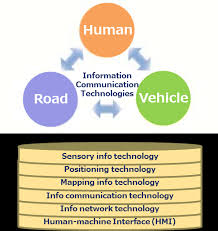
\includegraphics[width=0.45\textwidth]{images/ch1/components.png}%
     % you need to add the caption for the list of figures
    \caption[Components of ITS]{Components of ITS}\cite{web001}\label{fig: Components of ITS}%
  \end{figure}
  
  \hspace{2cm}The three most important components needed for establishing ITS are location, mapping, and communications.
An example of the component technology used for location includes the Global Positioning System (GPS). As GPS receivers have become quite inexpensive, they are now extensively used on familiar information devices, such as car navigation systems and mobile phones.
Mapping is a technology that plots location information on a map and can be realized with the help of a digital map.\cite{web001}


\section{Impact Of ITS}
Advantages of using intelligent transportation systems(ITS) systems are defined by various performance indicators. These indicators represent how ITS systems can improve the safety and mobility of the traveler, the efficiency of the transport system, performance of providers of transport services, energy-saving, and environmental protection. 
These measures include:
\begin{itemize}
    \item Safety: direct safety measures may include the number of accidents and changes in their number, the number of injuries and fatalities (absolute measurements). Direct relative measures can be analyzed as micro indicators (automotive, transportation, severity) specifying the number of events about the volume of traffic (miles traveled), the number of trips or proportion of involved fatalities or seriously injured persons in the total number of traffic incidents; and macro indicators (e.g. the density of accidents in the defined area or road section). Safety analyses also apply indirect measures which include traffic parameters and their dynamic range (e.g. vehicle speed, speed variation, changes in numbers of infringements of road safety traffic rules, rescue operation time, as well as drivers’ and pedestrians’ behavior measures). Safety can also be examined by defining social or individual risks .

    \item Mobility: these measures may include travel time, the variability of travel times (travel time reliability), variable speed (traffic flow), time to restore normal/typical traffic conditions (from the point of view of the user and efficiency of the transport system).

    \item Capacity: measured by the maximum number of people, goods or vehicles passing a point in the road (junction, perimeter or the reference point of the road network per unit of time), as well as traffic conditions (e.g. number of stops, number of vehicles/persons in the queues, time lost).

    \item Satisfaction of a service user (traveller, supplier of goods): related to the choice of means of transport and the quality of service measured by the level of satisfaction. Typical results of satisfaction with services provided include: assessment of professionalism of the service provided, meeting the traveller’s expectations, quality of use, as well as the level of service efficiency and reliability.

    \item Productivity: activities related to sufficient operational performance and security of the service costs .

    \item Energy and environment: measures include changes in the level of pollutant emissions (carbon dioxide and carbon monoxide, nitrogen oxides, hydrocarbons and volatile organic compounds) and energy consumption .
\end{itemize}

The efficiency of road traffic is closely related to the aforementioned indicators. Traffic performance is upgraded by increasing safety, improving mobility (reduction of travel time), increasing road capacity and use of public transport vehicles, reducing the cost of freight, reducing the negative impact of road traffic on the environment, as well as satisfaction of the road user (ITS services are to make, among other things, the journey more pleasurable and less tiresome).

The result of the implementation of ITS services can be a balance between all the indicators, e.g. improvement of the level of safety in such a way as not to cause a significant increase in travel time which translates directly into user satisfaction. On the other hand, the capacity should improve along with shortened travel time (taking into account all travellers, including cyclists and pedestrians) - but not at the expense of safety. In conclusion, the implementation of a new ITS service should consider comprehensively all aspects of traffic, so that the overall balance of such implementation was favourable, which requires developing methods defining such balance. \cite{web002}


\section{ITS Market Size}
\hspace{2cm}The global intelligent transportation system market size was valued at USD 26.58 billion in 2019 and is projected to register a compound annual growth rate (CAGR) of 5.8\% from 2020 to 2027. The necessity for presenting real-time traffic information of different regions to passengers and drivers is one of the significant factors driving the demand for intelligent transportation systems across the world. The growing number of vehicles on road, aging infrastructure, and lack of traffic data management are other factors anticipated to drive the overall growth. The need to enhance traffic flow across highways and corridors in cities has led to the rising need for an alternative technology to manage traffic. Transportation authorities can address the growing traffic issue by using innovative and advanced data analytic technologies.
\begin{figure}[htp]%
    \center%
    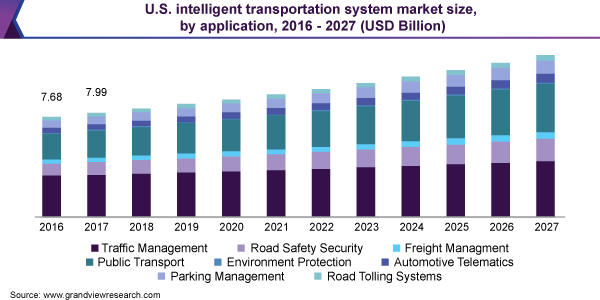
\includegraphics[width=1\textwidth]{images/ch1/us-intelligent-trITS-market.png}%
     % you need to add the caption for the list of figures
    \caption[ITS market size by applications]{ITS market size by applications}\cite{web003}\label{fig: ITS market size by applications}%
  \end{figure}
  
  High traffic jams owing to the increasing number of vehicles have contributed to the need for advanced public traffic management systems. Developments in emergency services and traffic management empower authorities to speedily respond to accidents and emergencies with more efficiency. The usage of such systems shortens the travel duration and increases efficiency in traffic management. The use of public transportation, such as buses and trains results in the reduction of carbon dioxide emissions and airborne pollutants.

Moreover, traffic congestion can be streamlined by deploying end-to-end connecting traffic management systems by using advanced techniques such as cloud computing and data analytic. Data collected from components such as sensors, video cameras, and embedded systems installed along the road can be used for analyzing and controlling real-time traffic across cities. Companies in the ITS market are conducting research and development activities to use data analytic and cloud to reduce congestion, improve traffic flow across various cities, reduce idle time, and improve fuel economy.

The logistics industry has been evolving with the advent of technology. Technologies, such as Artificial Intelligence (AI), Internet of Things (IoT), blockchain and big data, are rapidly transforming the way transportation systems are designed, planned, built, and operated. Logistics and transport involve a significant exchange of information and data between customers and service providers, and advances in information technology have been facilitating the rapid exchange of information and data. The latest technologies have enhanced visibility and control over shipments and subsequently augmented efficiency and customer satisfaction.

\begin{figure}[htp]%
    \center%
    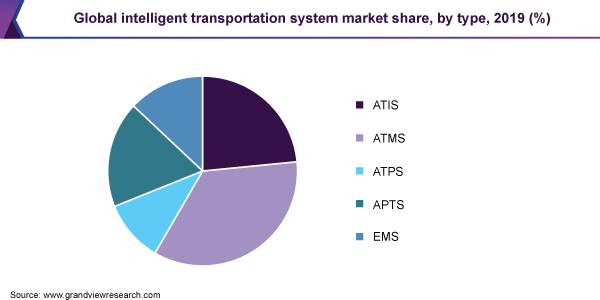
\includegraphics[width=1\textwidth]{images/ch1/global-market.png}%
     % you need to add the caption for the list of figures
    \caption[global market statics by types]{global market statics by types}\cite{web003}\label{fig: global market by types}%
  \end{figure}
  
 \textbf{Types of ITS application}
\begin{itemize}
\item Emergency Management System (EMS)
\item Advanced Traveler Information System (ATIS) 
\item Advanced Public Transportation System (APTS)
\item Advanced Transportation Pricing Systems (ATPS)
\item Advanced Traffic Management System (ATMS).
\end{itemize}
  
\hspace{2cm}Advanced Traffic Management System (ATMS) type segment led the market and accounted for more than 30.0\% share of the global revenue in 2019.

The advanced traffic management system primarily comprises applications for dynamic messaging signs, traffic signals, and ramp metering, among others. Bad traffic signal controls contribute considerably to congestion as well as an increase in the overall travel time to a large extent. ATMS helps in detecting dangerous weather conditions, roadway hazards, accidents, and creates a complete integrated view of overall traffic flow. They are installed with the present traffic control systems that generally help in reducing congestion and ensuring the efficient use of road space.\cite{web003}



\section{Advanced Public Transportation Systems}

\hspace{2cm}APTS are ITS technologies applied to public transit in order to improve operational efficiency, cost savings, safety, quality of service, and other transit measures of performance. Some APTS applications offer potential for improving service by providing greater leverage to service providers for managing and controlling bus transit operations. Other APTS applications provide benefits in terms of speed, security, and convenience directly to the customer. APTS have the potential to significantly change the way transit services are provided and the way customers use them.

The first examples of APTS date back to the late 1960s and early 1970s with the introduction of Automated Vehicle Monitoring (AVM) systems. The majority of these vehicle location technologies were signpost-based systems (with stationary signposts along bus routes). The signposts were equipped with electronic transmitters that emit unique identification codes. When a bus passed the signpost, an in-vehicle unit received the signpost’s identification code and record the time and date, the difference between the current odometer reading and the last (recorded at the previous signpost), and the vehicle’s identification code. The bus sent the information to the TOC via radio or other medium periodically or when prompted by the transit operations control center (TOC). Early implementations of APTS were expensive to install, operate, and maintain. Since then, new locations and communication technologies (e.g., GPS) have emerged and led to both improved performance and reduced costs.\cite{web004}

% Please add the following required packages to your document preamble:
% \usepackage{booktabs}
% \usepackage{graphicx}
\begin{longtable}{ |{h!}|p{9cm}|  }
\hline
 \textbf{Transit Application} & \textbf{APTS Technologies } \\
 \hline Fleet Management Systems &\begin{itemize}
 \item Automatic Vehicle Location Systems 
     \item Transit Operations Software 
     \item Communications Systems 
     \item Traffic Signal Priority Systems 
     \end{itemize} \\
 \hline
 Traveler  Information  Systems & \begin{itemize}
     \item Pre-Trip Transit and Multi-modal Traveler Information Systems
     \item In-Vehicle Transit Information Systems
 \end{itemize} \\
 \hline
 Electronic Payment Systems	& \begin{itemize}
     \item Smart Cards
     \item Fare Distribution Systems  
 \end{itemize}\\
 \hline
Transportation Demand Management &\begin{itemize}
     \item Dynamic Ride-sharing
     \item Automated Service Coordination 
     \item Transportation Management Centers 
 \end{itemize} \\
 \hline
\caption{APTS technologies for transit application}
\label{APTS technologies}
\end{longtable}

\textbf{Fleet Management Systems:}focus on improving the planning, scheduling, and operations of a fleet of vehicles. The related strategies aim at improved service reliability, safety, and operating efficiency (e.g., reduced non revenue time, increased productivity) and faster service disruption recovery. In general, fleet management includes technologies that collect and make available vehicle performance data (e.g., vehicle location), and technologies that use that data for real-time control or for planning and scheduling. Important technologies used for fleet management purposes include: Communications Systems, Geographic Information Systems (GIS), Automated Vehicle Location Systems (AVL), Automatic Passenger Counters (APC), Transit Operations Software, and Traffic Signal Priority.

\textbf{Traveler Information Systems} refers to technologies used to provide travel information to passengers in order to assist their trip-making decision. The information provided may range from static route, schedule, and fare information to real-time vehicle location and/or estimated arrival time. AVL systems are the enabler for the provision of real-time information. Traveler information may be disseminated through various means, for example, web-based itinerary planning services, smart phones, in-vehicle units, etc. Traveler information is generally expected to improve the quality of transit service by improving the passenger experience. Traveler information may give passengers a better sense of control over their trip-making decisions and/or enable them to take action to minimize waiting times at stops, plan transfer connections, and thus reduce overall travel time. Information may be provided prior to departure (e.g., by phone, internet), at the terminal or stop, or in the transit vehicle. Information influences passenger trip-making decisions, for example, route, stop, departure time choice, etc. The attractiveness of transit alternatives is a function of waiting time, in-vehicle travel time, transfer time to the connecting trip, number of transfers, on board comfort (crowding), etc. Information systems can provide timely information regarding many of these attributes.

\textbf{Electronic Payment Systems} forego cash and token payment with the aim of reducing the operating costs of fare collection systems, increasing safety and security on the vehicle, improving data collection, and increasing customer convenience . There are several electronic fare payment technologies, including magnetic stripe cards, and smart cards. Electronic fare payment technologies can have significant impacts on transit operations. The most obvious of the potential impacts on operations occur at the bus stop, where passengers board and alight from the vehicle. Depending on the type of electronic fare payment technology, considerable gains can be realized in terms of lower dwell times at stops through increased transaction speeds. Contact card technologies, where the card is physically swiped through a card reader, and contact less card technologies, where the card and card reader communicate without physical contact but rather via an electromagnetic signal, affect passenger boarding rates differently. Boarding rates increase to a greater extent with contact less card technologies.

\textbf{Transportation Demand Management} is the application of technology to alter the usage patterns of the transportation network, with an emphasis on encouraging users to travel by transit. There is a broad range of technologies designed to better coordinate various transit services, and provide forums for organized carpooling and car sharing . In general, approaches to managing transportation demand aim at increasing the number of high occupancy vehicles in congested transportation networks, promote travel in off-peak hours, and implementing transit incentive programs. Examples include dynamic ride sharing and automated service coordination.\cite{web004}


\section{Project Scope}


\hspace{2cm} Transportation is a daily need that we all require whether to go schooling, work, make a visit or even do shopping . In a country as Egypt with a broad population segment living on the public buses and micro-buses, it is a matter of millions to help them get a better transportation service that is at least more organized.
At the main stations, buses -for example- take long time to get a complete number of passengers to move their way while many of them are already waiting for a ride in the road to the bus’s final destination. This situation makes the bus get too much time waiting people, and on the other hand, the people are waiting for the bus miles or some away from the station. So, this project offers an advanced service for both the bus-drivers and the people waiting them. It allows the main user to register with his location and the user to book a seat or more according to their number so the bus-driver take off from the station with seats of their number unoccupied. 
This mobile app has a double-benefit relationship for the two kind of users due to the multi-featured software. 

Our work to complete this project is divided into three milestones:
\begin{itemize}

\item \textbf{Develop a mobile-app (klax) for users which features}:
    \begin{itemize}
    \item booking a trip at specific time .
    \item selecting his line and station .
    \item identify source && destination location for user .
    \item optimizing nearest station to pick-up. 
    \item selecting number of seats (max 5 seats).
    \item tracking driver and knowing time for pick up.
    \item booking a trip for other people.
    \item tracking his family accounts and trips for safety .
    \item paying trip cost by vise or cash .
    \item editing profile page for user.
    \item booking a private trip .
    \item sending feedback
    \end{itemize}
\item \textbf{Develop a mobile-app (klax) for drivers which features}:
    \begin{itemize}
        \item uploading information about him(photo, licence, address,..) ,his car (color ,car number,car licence,) and lines where work.
        \item receiving requests from users.
        \item tracking user locations .
        \item following balance .
        \item statics about number of trips and profit .
        \item sending and receiving feedback about trips.
    \end{itemize}
\item \textbf{Develop a web server to perform the following tasks}:
    \begin{itemize}
    \item Monitoring users, drivers and trip numbers.
    \item Geographic distribution of passengers according to their governs.
    \item Application monthly revenue.
    \item Making new offers and promo codes to users ( discounts, free trips, free cash).
    \item Viewing passenger information.
    \item Getting every driver live location and make sure he is committed to his route.
    \item Viewing passengers complaints and send response.
    \item Adding lines and stations to the application whenever we decide.
    \end{itemize}
    

\end{itemize}